\subsection{Overview}

    \begin{figure}[H]
        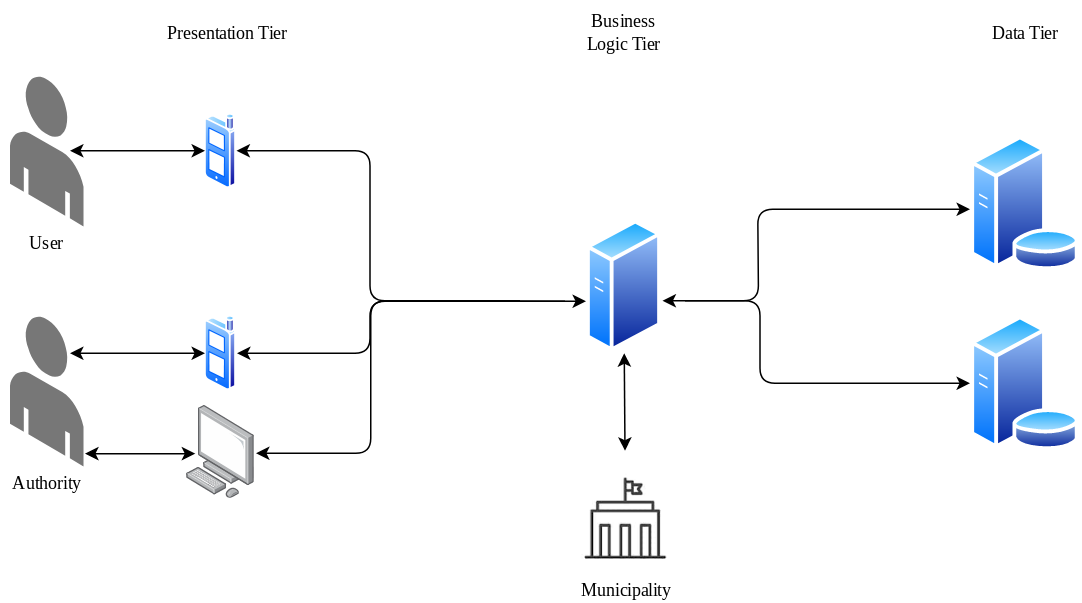
\includegraphics[width=\textwidth]{Images/SystemOverview.png}
        \caption{\label{fig:SystemOverview}High level overwiew of the system}
    \end{figure}
   
\newpage

\subsection{Component View}

    \begin{figure}[H]
        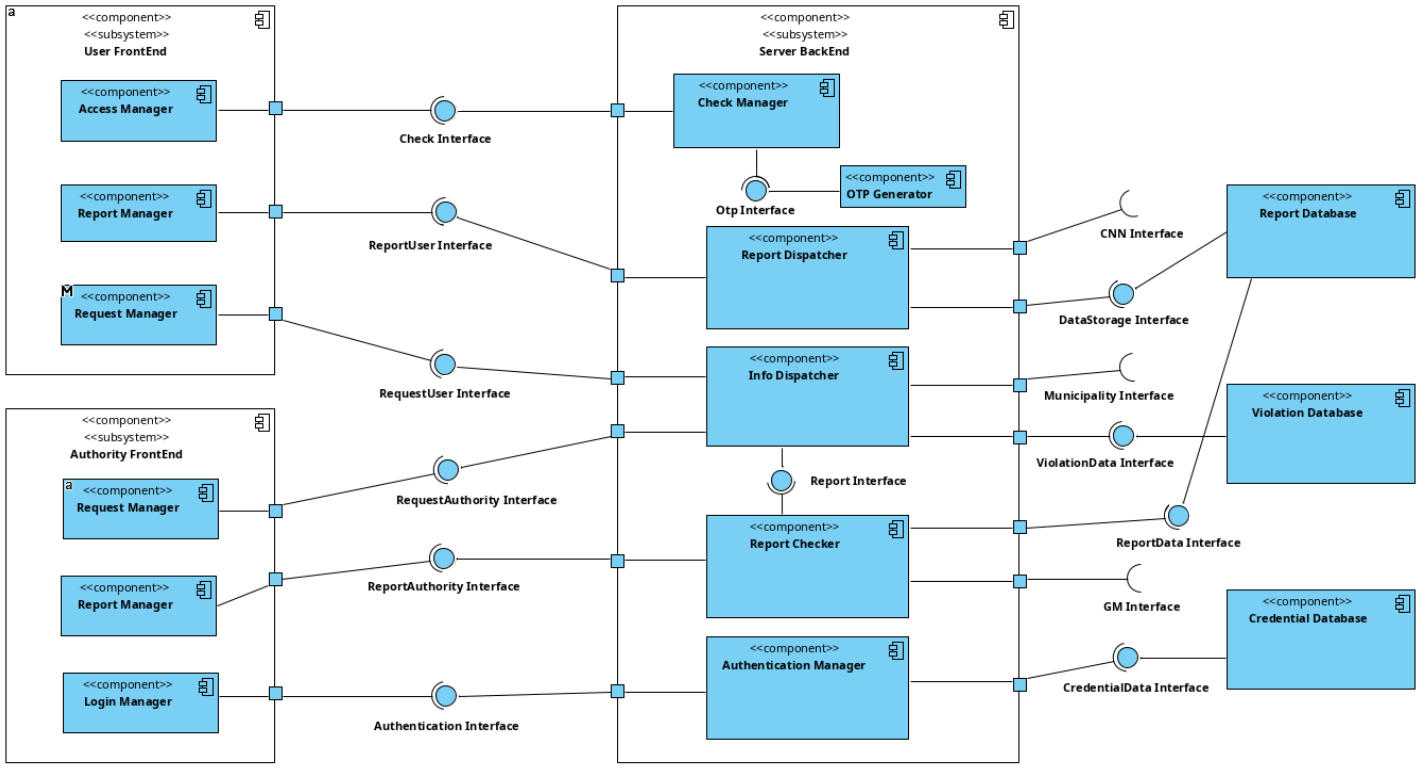
\includegraphics[width=\textwidth]{Images/ComponentView.png}
        \caption{\label{fig:ComponentView}Component diagram}
    \end{figure}

    The UML Component diagram shows the internal modular 
    structure of the components and their connections. 
    To communicate, they can require a variable number 
    of interfaces and attributes. 
    A brief description of each component, w.r.t the 
    most importants interfaces, is presented:

    \begin{itemize}

        \item Clients: Users' and authorities' machines, they 
        can be either mobile devices or computers.
        
        \begin{itemize}

            \item User Frontend

            \begin{itemize}

                \item Report Manager: Establishes an exchange 
                of messages with the Server and sends data 
                regarding the alleged violation, to be 
                later examined.
                
                \item Request Manager: Retrieves the list of 
                violations or accidents using the Server.
                
            \end{itemize}

            \item Authority Frontend

            \begin{itemize}

                \item Report Manager: Retrieves a report and 
                orders to approve it or to discard it, 
                based on the information stored.
                
                \item Request Manager: Retrieves the list 
                of violations or accidents using the Server.
                
            \end{itemize}
            
        \end{itemize}

        \item Server Backend: Interacts with the clients and 
        the Databases and contains the logic of the Application.
        
        \begin{itemize}
            \item Check Manager: Requests and receives the OTP 
            by OTPGenerator to withstand the login of the user.
            
            \item Report Dispatcher: Receives the information 
            about the reports filed by users and pushes them 
            to the Report Server if the report is correctly 
            fulfilled, aborting the incorrect ones.

            \item Authentication Manager: Exchanges information 
            with the Database containing the credentials of the 
            authority that wants to login and ultimates the 
            login process.
            
            \item Info Dispatcher: Communicates with both the 
            types of users to retrieve information about 
            violations or accidents (these are retrieved by 
            the Municipality API). \textit{Note: different 
            kinds of users receive different quantities of 
            information, for example, users do no obtain 
            the license plates of the offenders.}

            \item Report Checker: Sends information about the 
            open reports to AuthorityFrontend/ReportManager, 
            locates the position using GM API and receives 
            the approval of dismissal of said reports to store 
            them as Violations on the Violation Database 
            or not, by sending them to InfoDispatcher.

        \end{itemize}
        
        \item Databases: They allow the retrieval and addition 
        of data.
        
    \end{itemize}

\newpage



\subsection{Deployment View}

    \begin{figure}[H]

        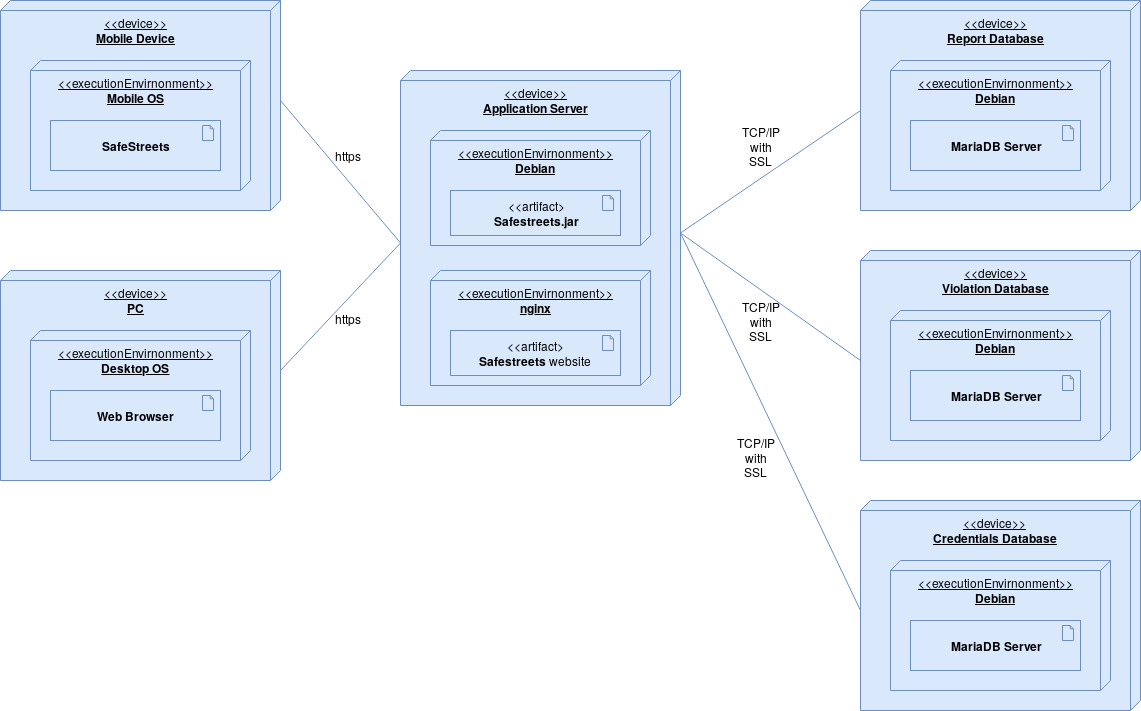
\includegraphics[width=\textwidth]{Images/deployment.jpg}
        \caption{\label{fig:deployment}Deployment diagram}
        
    \end{figure}
	
    The purpose of the Deployment diagram is to specify the distribution 
    of the components of the system, showing the configuration of run 
    time processing nodes and components that live on them. 

\newpage

\subsection{Runtime View}
\subsubsection{User Access}
	\begin{figure}[H]
		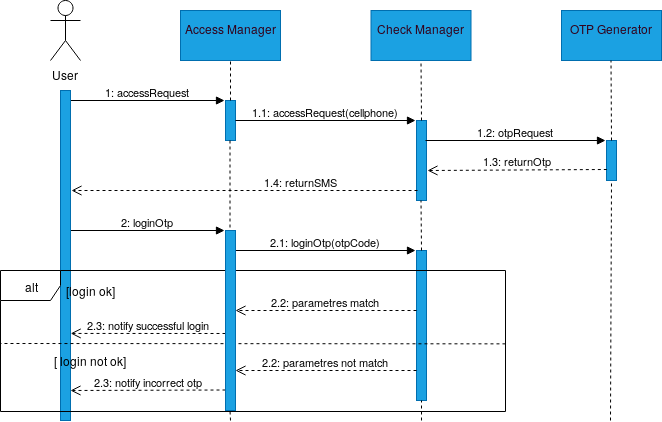
\includegraphics[width=\textwidth]{Images/RunTimeViewUserAccess.png}		
		\caption{\label{fig:UserAccess}User access sequence diagram}
	\end{figure}
\subsubsection{Authority Access}
	\begin{figure}[H]
		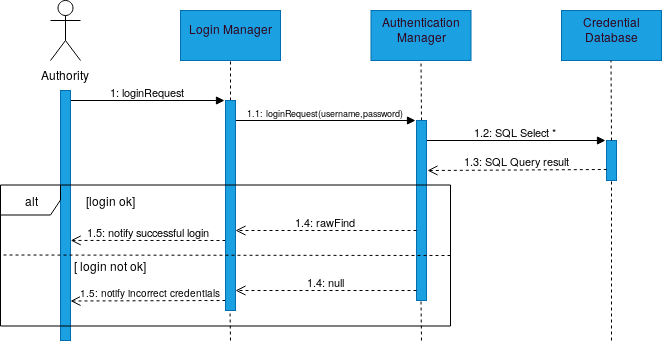
\includegraphics[width=\textwidth]{Images/RunTimeViewAuthorityAccess.png}
		\caption{\label{fig:AuthorityAccess}Authority access sequence diagram}	
	\end{figure}
\subsubsection{User Files a report}
	\begin{figure}[H]
		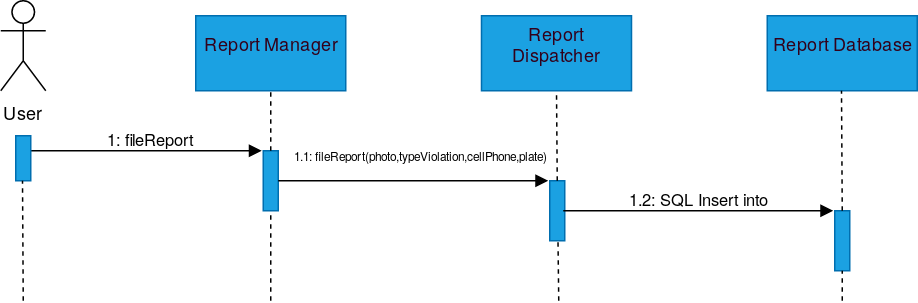
\includegraphics[width=\textwidth]{Images/RunTimeViewUserReport.png}		
		\caption{\label{fig:UserReport}User files a report sequence diagram}
	\end{figure}
\subsubsection{Authority Checks a report}
	\begin{figure}[H]
		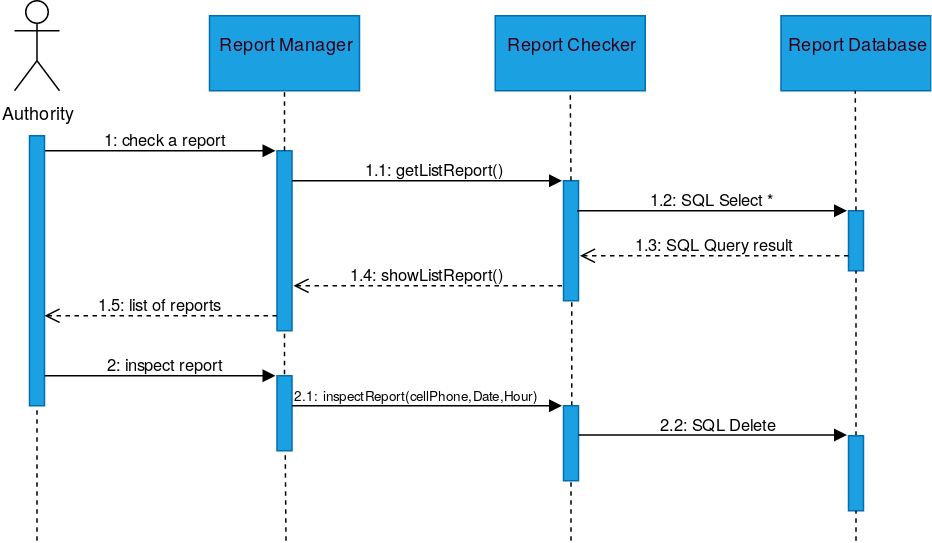
\includegraphics[width=\textwidth]{Images/RunTimeViewAuthorityCheck.png}		
		\caption{\label{fig:UserReport}Authority checks a report sequence diagram}
	\end{figure}
\subsubsection{Authority/User reads list of violations}
	\begin{figure}[H]
		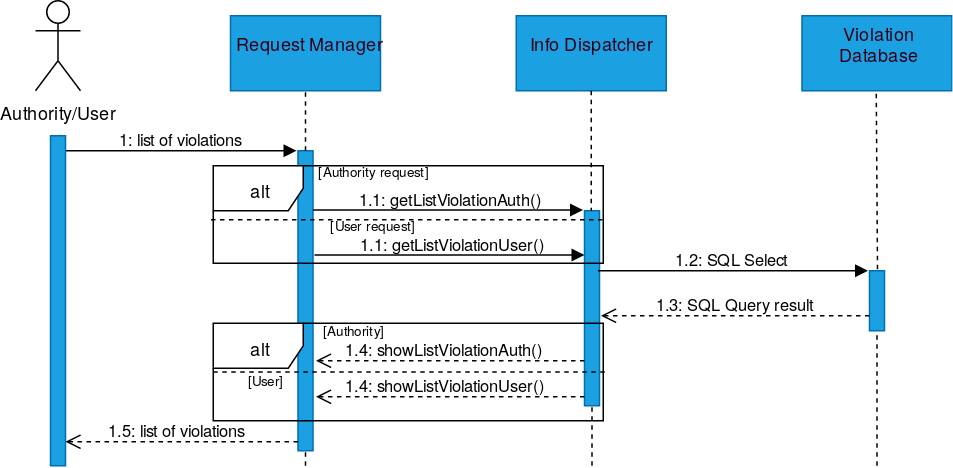
\includegraphics[width=\textwidth]{Images/RunTimeViewListViolation.png}		
		\caption{\label{fig:UserReport}Authority/User reads list of violations sequence diagram}
	\end{figure}

\newpage
\subsection{Component Interfaces}
\begin{figure}[H]
		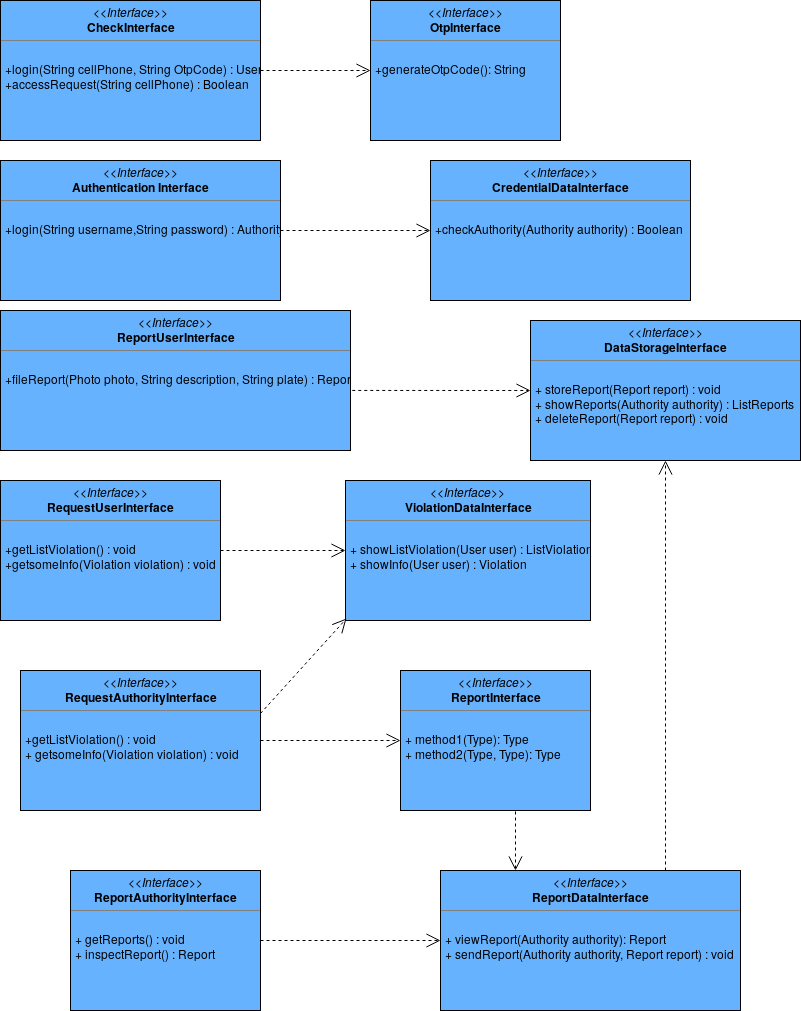
\includegraphics[width=\textwidth]{Images/ComponentInterfaces.png}		
		\caption{\label{fig:ComponentInterfaces}Component Interfaces}
	\end{figure}
\newpage
\subsection{Selected architectural styles and patterns}

\subsubsection{Three Tier client-server}

The architectural style chosen for Safestreets is the 
\textbf{client-server} in its \textbf{three-tier} variant.  
It allows the separation of the access to data, 
presentation and logic of the application.
The main advantage of a multilayered architecture 
is the decoupling of Logic and Data. This leads to a high 
level of Mantainability and Scalability, 
qualities that are extremely useful when working with 
cities that tend to expand their territory and consequently 
the number of streets to be controlled.
At the same time the system is safe as the access to data 
is transparent to the end user.

\subsubsection{MVC}

MVC is a desing pattern that breaks an application into 
different layers of functionalities: Model, View and 
Controller.
This allows for the internal representation of 
information to differ from the information presented 
to the user. 
This produces easily reusable and flexible code 
and allows parallel development. 

\texttt{The division:}

\begin{itemize}
    \item \textbf{View:} Clients.
    \item \textbf{Controller:} Application.
    \item \textbf{Model:} DBs.
    
    
\end{itemize}

\subsection{Other Design Decisions}

\subsubsection{Thin Client}

In SafeStreets the client contains no logic of the 
Application at all, but it is just able to format 
and send reports and to request lists.
This guarantees the App to be "light" on resources 
and power consumption (users do not need to 
have a high end smartphone) while keeping it easily 
upgradable.

\subsubsection{Data Division}

Data is spread among three different DBs as 
different types of data requires different levels 
of security and replication:

\begin{itemize}

    \item  Report Databse: The data saved on this 
    DB is not important as reports are very dependent 
    on time. The images and information stored are not 
    legally binding (only authorities can administer 
    fines), thus it must be able to handle large 
    quantities of data and be operative in a short 
    span of time but data loss can be sustained.

    \item Violation Database: The data stored here 
    is composed of light elements (only text) 
    which do not require particular encryption 
    thus the server is able to sustain a great 
    deal of ACID operations but requires data 
    duplication.

    \item Credentials Database: This DB contains 
    information for the Authentication of the 
    authorities so, not only does it require data 
    duplication to be quickly operative also in 
    case of failure, but encryption is also 
    crucial to this device. Data is stored 
    following good pratices of security (e.g. 
    only the salted hashes of the password are 
    saved).     

\end{itemize}